% !TEX TS-program = XeLaTeX
% use the following command:
% all document files must be coded in UTF-8
\documentclass[spanish]{textolivre}
% build HTML with: make4ht -e build.lua -c textolivre.cfg -x -u article "fn-in,svg,pic-align"

\journalname{Texto Livre}
\thevolume{16}
%\thenumber{1} % old template
\theyear{2023}
\receiveddate{\DTMdisplaydate{2022}{9}{24}{-1}} % YYYY MM DD
\accepteddate{\DTMdisplaydate{2022}{11}{21}{-1}}
\publisheddate{\DTMdisplaydate{2023}{1}{18}{-1}}
\corrauthor{Ricardo-Adán Salas-Rueda}
\articledoi{10.1590/1983-3652.41293}
%\articleid{NNNN} % if the article ID is not the last 5 numbers of its DOI, provide it using \articleid{} commmand 
% list of available sesscions in the journal: articles, dossier, reports, essays, reviews, interviews, editorial
\articlesessionname{articles}
\runningauthor{Salas-Rueda et al.} 
%\editorname{Leonardo Araújo} % old template
\sectioneditorname{Hugo Heredia Ponce}
\layouteditorname{Thaís Coutinho}

\title{Uso de los algoritmos Machine Learning para analizar Moodle y los teléfonos inteligentes en el proceso educativo de la Física}
\othertitle{Uso dos algoritmos Machine Learning para analisar o Moodle e os telefones inteligentes no processo educativo da Física}
\othertitle{Use of Machine Learning algorithms to analyze Moodle and smartphones in the educational process of Physics}
% if there is a third language title, add here:
%\othertitle{Artikelvorlage zur Einreichung beim Texto Livre Journal}

\author[1]{Ricardo-Adán Salas-Rueda~\orcid{0000-0002-4188-4610}\thanks{Email: \href{mailto:ricardo.salas@icat.unam.mx}{ricardo.salas@icat.unam.mx}}}
\author[1]{Jesús Ramírez-Ortega~\orcid{0000-0002-4538-9203}\thanks{Email: \href{mailto:jesus.ramirez@icat.unam.mx}{jesus.ramirez@icat.unam.mx}}}
\author[1]{Selene-Marisol Martínez-Ramírez~\orcid{0000-0002-5655-0963}\thanks{Email: \href{mailto:selene.martinez@icat.unam.mx}{selene.martinez@icat.unam.mx}}}
\author[1]{Clara Alvarado-Zamorano~\orcid{0000-0001-9122-7590}\thanks{Email: \href{mailto:clara.alvarado@icat.unam.mx}{clara.alvarado@icat.unam.mx}}}
\affil[1]{Universidad Nacional Autónoma de México, Instituto de Ciencias Aplicadas y Tecnología, Ciudad de México, México.}

\addbibresource{article.bib}
% use biber instead of bibtex
% $ biber article

% used to create dummy text for the template file
\definecolor{dark-gray}{gray}{0.35} % color used to display dummy texts
\usepackage{lipsum}
\SetLipsumParListSurrounders{\colorlet{oldcolor}{.}\color{dark-gray}}{\color{oldcolor}}

% used here only to provide the XeLaTeX and BibTeX logos
\usepackage{hologo}

% if you use multirows in a table, include the multirow package
\usepackage{multirow}

% provides sidewaysfigure environment
\usepackage{rotating}

% CUSTOM EPIGRAPH - BEGIN 
%%% https://tex.stackexchange.com/questions/193178/specific-epigraph-style
\usepackage{epigraph}
\renewcommand\textflush{flushright}
\makeatletter
\newlength\epitextskip
\pretocmd{\@epitext}{\em}{}{}
\apptocmd{\@epitext}{\em}{}{}
\patchcmd{\epigraph}{\@epitext{#1}\\}{\@epitext{#1}\\[\epitextskip]}{}{}
\makeatother
\setlength\epigraphrule{0pt}
\setlength\epitextskip{0.5ex}
\setlength\epigraphwidth{.7\textwidth}
% CUSTOM EPIGRAPH - END

% LANGUAGE - BEGIN
% ARABIC
% for languages that use special fonts, you must provide the typeface that will be used
% \setotherlanguage{arabic}
% \newfontfamily\arabicfont[Script=Arabic]{Amiri}
% \newfontfamily\arabicfontsf[Script=Arabic]{Amiri}
% \newfontfamily\arabicfonttt[Script=Arabic]{Amiri}
%
% in the article, to add arabic text use: \textlang{arabic}{ ... }
%
% RUSSIAN
% for russian text we also need to define fonts with support for Cyrillic script
% \usepackage{fontspec}
% \setotherlanguage{russian}
% \newfontfamily\cyrillicfont{Times New Roman}
% \newfontfamily\cyrillicfontsf{Times New Roman}[Script=Cyrillic]
% \newfontfamily\cyrillicfonttt{Times New Roman}[Script=Cyrillic]
%
% in the text use \begin{russian} ... \end{russian}
% LANGUAGE - END

% EMOJIS - BEGIN
% to use emoticons in your manuscript
% https://stackoverflow.com/questions/190145/how-to-insert-emoticons-in-latex/57076064
% using font Symbola, which has full support
% the font may be downloaded at:
% https://dn-works.com/ufas/
% add to preamble:
% \newfontfamily\Symbola{Symbola}
% in the text use:
% {\Symbola }
% EMOJIS - END

% LABEL REFERENCE TO DESCRIPTIVE LIST - BEGIN
% reference itens in a descriptive list using their labels instead of numbers
% insert the code below in the preambule:
%\makeatletter
%\let\orgdescriptionlabel\descriptionlabel
%\renewcommand*{\descriptionlabel}[1]{%
%  \let\orglabel\label
%  \let\label\@gobble
%  \phantomsection
%  \edef\@currentlabel{#1\unskip}%
%  \let\label\orglabel
%  \orgdescriptionlabel{#1}%
%}
%\makeatother
%
% in your document, use as illustraded here:
%\begin{description}
%  \item[first\label{itm1}] this is only an example;
%  % ...  add more items
%\end{description}
% LABEL REFERENCE TO DESCRIPTIVE LIST - END


% add line numbers for submission
%\usepackage{lineno}
%\linenumbers

\begin{document}
\maketitle

\begin{polyabstract}
\begin{abstract}
El objetivo de este estudio mixto es analizar las percepciones de los alumnos sobre el uso de Moodle y los teléfonos inteligentes en el proceso educativo de la Física a través de la Ciencia de Datos. Los algoritmos Machine Learning utilizados son regresión lineal, árbol de decisión y deep learning. En este estudio, la incorporación de Moodle facilitó la entrega de tareas, la consulta de los contenidos, la comunicación y la revisión de los recursos multimedia. Incluso, los teléfonos inteligentes permitieron el acceso a las plataformas virtuales de aprendizaje, el uso de las aplicaciones móviles y la comunicación desde cualquier lugar. Los resultados de los algoritmos regresión lineal y deep learning indican que el uso de Moodle y los teléfonos inteligentes influye positivamente la motivación de los alumnos, la asimilación del conocimiento y la satisfacción en el curso Física. Por otro lado, el algoritmo árbol de decisión determina 6 modelos predictivos. Las limitaciones son las técnicas de Machine Learning utilizadas y el análisis de las herramientas tecnológicas para la asimilación del conocimiento, la motivación y la satisfacción. Los futuros estudios pueden analizar el uso de Moodle y los teléfonos inteligentes para el rol activo y el desarrollo de las habilidades en diversas preparatorias y universidades. Asimismo, los algoritmos Machine Learning sobre los bosques aleatorios y la regresión logística pueden ser empleados para analizar el impacto de estas herramientas tecnológicas considerando el rendimiento académico. Por último, la incorporación de Moodle y los teléfonos inteligentes permite actualizar los cursos y diseñar creativas actividades a distancia.

\keywords{Moodle \sep Teléfonos inteligentes \sep Aprendizaje máquina \sep Aprendizaje profundo \sep Educación}
\end{abstract}

\begin{portuguese}
\begin{abstract}
O objetivo deste estudo misto é analisar as percepções dos alunos sobre o uso do Moodle e smartphones no processo educacional de Física por meio da Ciência de Dados. Os algoritmos de Machine Learning utilizados são regressão linear, árvore de decisão e deep learning. Neste estudo, a incorporação do Moodle facilitou a entrega de tarefas, a consulta dos conteúdos, a comunicação e a revisão dos recursos multimédia. Os smartphones permitiram ainda o acesso a plataformas virtuais de aprendizagem, a utilização de aplicações móveis e a comunicação a partir de qualquer lugar. Os resultados dos algoritmos de regressão linear e deep learning indicam que o uso do Moodle e smartphones influencia positivamente a motivação dos alunos, a assimilação do conhecimento e a satisfação no curso de Física. Por outro lado, o algoritmo da árvore de decisão determina 6 modelos preditivos. As limitações são as técnicas de Machine Learning utilizadas e a análise de ferramentas tecnológicas para a assimilação do conhecimento, motivação e satisfação. Estudos futuros podem analisar o uso do Moodle e smartphones para papel ativo e desenvolvimento de habilidades em várias escolas de ensino médio e universidades. Da mesma forma, algoritmos de Machine Learning sobre florestas aleatórias e regressão logística podem ser usados para analisar o impacto dessas ferramentas tecnológicas no desempenho acadêmico. Por último, a incorporação do Moodle e dos smartphones permite a atualização dos cursos e o desenho de atividades criativas à distância.

\keywords{Moodle \sep Smartphones \sep Aprendizado de máquina \sep Aprendizagem profunda \sep Educação}
\end{abstract}
\end{portuguese}

\begin{english}
\begin{abstract}
The aim of this mixed study is to analyze the students' perceptions on the use of Moodle and smartphones in the educational process about Physics through Data Science. The algorithms of Machine Learning used are linear regression, decision tree and deep learning. In this research, the incorporation of Moodle facilitated the delivery of tasks, consultation of contents, communication and review of multimedia resources. Likewise, smartphones allowed the access to virtual learning platforms, use of mobile applications and communication from anywhere. The results of the linear regression and deep learning algorithms establish that the use of Moodle and smartphones positively influence the motivation of the students, assimilation of knowledge and satisfaction in the Physics course. On the other hand, the decision tree algorithm determines 6 predictive models. The limitations are the Machine Learning techniques used and the analysis of technological tools for the assimilation of knowledge, motivation and satisfaction. Future studies may look at the use of Moodle and smartphones for active role and skill development in various high schools and universities. Likewise, Machine Learning algorithms on random forests and logistic regression can be used to analyze the impact of these technological tools considering academic performance. Finally, the incorporation of Moodle and smartphones allows updating the courses and designing creative distance activities.

\keywords{Moodle \sep Smartphones \sep Machine learning \sep Deep learning \sep Education}
\end{abstract}
\end{english}
% if there is another abstract, insert it here using the same scheme
\end{polyabstract}

\section{Introducción}\label{sec-intro}
Las instituciones educativas enfrentan el reto de cambiar las actividades de los cursos a través de las Tecnologías de la Información y Comunicación (TIC) y los modelos pedagógicos \cite{gormaz-lobos_evaluation_2021, heethal_jaiprakash_flipped_2022, koyuncu_classification_2022}. Los sistemas de gestión de aprendizaje, las herramientas en la nube Google, los sistemas de videoconferencia, los dispositivos móviles y las herramientas Web 2.0 permitieron la enseñanza y el aprendizaje durante el periodo del COVID-19 \cite{karahisar_research_2022, koyuncu_classification_2022}.

Las ventajas relacionadas con la implementación de la educación a distancia son el aprendizaje personalizado, la reducción de costos, la autonomía, el acceso a los cursos y la revisión de los recursos multimedia desde cualquier lugar \cite{farsi_investigating_2022, karahisar_research_2022}. De hecho, los docentes se apoyan en los sistemas de gestión de aprendizaje y los dispositivos móviles para facilitar el rol activo de los estudiantes durante el proceso educativo \cite{farsi_investigating_2022, galarce-miranda_analysis_2022, verawati_enhancing_2022}.

Los sistemas de gestión de aprendizaje como Moodle, Blackboard y Google Classroom permiten que los alumnos realicen los exámenes en línea, consulten los contenidos, participen en los foros de discusión y entreguen las tareas \cite{farsi_investigating_2022, galarce-miranda_analysis_2022}. Por otro lado, los dispositivos móviles como los teléfonos inteligentes, las computadoras portátiles y las tabletas facilitan el acceso a los sistemas de gestión de aprendizaje, el empleo de las herramientas tecnológicas, la búsqueda de información en Internet y la comunicación \cite{farsi_investigating_2022, rysbayeva_students_2022, verawati_enhancing_2022}.

La Ciencia de Datos tiene un papel fundamental durante el análisis sobre el comportamiento de los fenómenos educativos \cite{chadaga_battling_2021, khakpour_convergence_2021, salas-rueda_use_2021}. En particular, los algoritmos Machine Learning como la regresión lineal y árbol de decisión permiten identificar información nueva para la toma de decisiones en el campo educativo \cite{alenezi_utilizing_2020, khakpour_convergence_2021}.

Por ejemplo, la técnica regresión lineal determinó el impacto sobre la consulta de videos y el uso de Google Drive en el curso Matemáticas Financieras \cite{salas-rueda_use_2021}. Del mismo modo, la técnica árbol de decisión permitió identificar las condiciones que influyen el proceso de enseñanza-aprendizaje sobre la informática antes, durante y después de las sesiones presenciales a través del uso del software MYSQL y la revisión de los videos YouTube \cite{salas-rueda_use_2020}.

Durante el COVID-19, la Universidad Nacional Autónoma de México (UNAM) en los niveles medio y superior modificó la forma de impartir sus cursos, es decir, las herramientas tecnológicas adquirieron un papel indispensable para realizar el proceso de enseñanza y aprendizaje de forma virtual. Por consiguiente, el educador de la asignatura Física en la Escuela Nacional Preparatoria no. 6 decidió incorporar Moodle y los teléfonos inteligentes en las actividades durante el ciclo escolar 2021.

En este estudio, la incorporación de Moodle facilitó la entrega de tareas, la consulta de los contenidos, la revisión de los recursos multimedia y la comunicación. Incluso, los teléfonos inteligentes permitieron el acceso a las plataformas virtuales de aprendizaje, el uso de las aplicaciones móviles y la comunicación desde cualquier lugar.

El objetivo de este estudio mixto es analizar las percepciones de los alumnos sobre el uso de Moodle y los teléfonos inteligentes en el proceso educativo de la Física a través de la Ciencia de Datos. Los algoritmos Machine Learning utilizados son regresión lineal, árbol de decisión y deep learning. A continuación, se presentan las preguntas de investigación:

\begin{itemize}
  \item ¿Cuál es la percepción de los participantes sobre el uso de Moodle y los teléfonos inteligentes para la motivación, la asimilación del conocimiento y la satisfacción en el curso Física considerando los algoritmos regresión lineal y deep learning?
  \item ¿Cuáles son las condiciones predictivas sobre el uso de Moodle y los teléfonos inteligentes considerando el algoritmo árbol de decisión?
  \item ¿Cuál es la percepción de los alumnos sobre el uso de Moodle y los teléfonos inteligentes en el campo educativo de la Física?
\end{itemize}


\section{Revisión de Literatura}

\subsection{Ciencia de Datos}

Hoy en día, la Ciencia de Datos permite encontrar nuevos patrones para clasificar y evaluar la información \cite{chadaga_battling_2021, khanal_systematic_2020}. De hecho, el uso de los algoritmos Aprendizaje Automático o Machine Learning ayuda a tomar una mejor decisión a través de la predicción de los fenómenos \cite{chadaga_battling_2021, khanal_systematic_2020, koyuncu_classification_2022}.

En el Machine Learning, los algoritmos supervisados como la regresión lineal, el árbol de decisión, los bosques aleatorios, las redes neuronales artificiales, las máquinas de vectores de soporte y la regresión logística facilitan el descubrimiento de nuevos datos \cite{chadaga_battling_2021}.

El algoritmo Machine Learning sobre la regresión lineal ayuda a evaluar las hipótesis a través de la división de la muestra \cite{alenezi_utilizing_2020, chadaga_battling_2021, khakpour_convergence_2021}. La sección entrenamiento determina las funciones y la sección evaluación identifica la exactitud de éstas \cite{khakpour_convergence_2021}. Por ejemplo, el uso del algoritmo regresión lineal facilitó el análisis sobre la incorporación de los juegos digitales, el rendimiento académico, el desarrollo de habilidades, la motivación y el aprendizaje personalizado \cite{khakpour_convergence_2021}.

Del mismo modo, los algoritmos Machine Learning (regresión lineal y árbol de decisión) facilitaron la predicción del rendimiento académico a través de los sistemas de gestión de aprendizaje \cite{koyuncu_classification_2022}. De hecho, el algoritmo árbol de decisión permite encontrar las relaciones y condiciones entre los fenómenos de estudio con el propósito de predecir los eventos \cite{alenezi_utilizing_2020, chadaga_battling_2021, skrbinjek_predicting_2019}.

En el campo educativo, el algoritmo árbol de decisión determinó las condiciones y los modelos predictivos sobre la ejecución de las actividades a distancia y el rendimiento académico \cite{skrbinjek_predicting_2019}. Por otro lado, el algoritmo deep learning permite identificar los modelos predictivos más eficientes para el análisis y la predicción de los fenómenos educativos \cite{doleck_predictive_2020}.

Por último, la Ciencia de Datos con el apoyo de los algoritmos Machine Learning facilitan el modelado de los fenómenos a través de la evaluación y clasificación de los eventos \cite{alenezi_utilizing_2020, chadaga_battling_2021, khanal_systematic_2020}.


\subsection{Uso de herramientas tecnológicas durante el COVID-19}
Debido al virus SARS-CoV-2, los educadores necesitaron actualizar las actividades escolares para realizar la educación a distancia \cite{farsi_investigating_2022, stevanus_impact_2022}. En Irán, los estudiantes de Enfermería utilizaron el sistema de videoconferencia SkyRoom, el sistema de gestión de aprendizaje llamado NAVID, los videos YouTube, las presentaciones digitales y los dispositivos móviles para facilitar la comprensión de los temas clínicos durante el COVID-19 \cite{farsi_investigating_2022}.

En la República Democrática del Congo, los dispositivos móviles, Zoom y los sistemas de gestión de aprendizaje como Moodle y Blackboard facilitaron la realización del proceso educativo en las universidades y preparatorias bajo la modalidad Blended Learning \cite{kiketa_design_2022}. Del mismo modo, los alumnos de las universidades en Kazakhstan incrementaron su motivación y comprendieron los temas de los cursos desde cualquier lugar a través de las aplicaciones móviles \cite{rysbayeva_students_2022}.

En la Universidad de Mataram, los sistemas de gestión de aprendizaje y los dispositivos móviles facilitaron el proceso de aprendizaje virtual \cite{verawati_enhancing_2022}. Según los estudiantes del curso Ingeniería, los teléfonos inteligentes son una herramienta tecnológica ideal para la asimilación del conocimiento en cualquier momento y la resolución de los problemas a través de las aplicaciones móviles \cite{omirzak_students_2021}.

Por último, las herramientas tecnológicas permitieron enfrentar los retos originados por el virus SARS-CoV-2 debido a que éstas facilitaron la revisión de la información, la consulta de los recursos multimedia, la realización de actividades y el establecimiento efectivo de la comunicación \cite{galarce-miranda_analysis_2022, gormaz-lobos_evaluation_2021, stevanus_impact_2022}.


\section{Metodología}
Los objetivos particulares de este estudio son: 1. Analizar el uso de Moodle y los teléfonos inteligentes para la motivación de los participantes, la asimilación del conocimiento y la satisfacción en el curso Física por medio de los algoritmos regresión lineal y deep learning, 2. Establecer las condiciones predictivas (modelos) sobre Moodle, las características de los estudiantes y los teléfonos inteligentes a través del algoritmo árbol de decisión y 3. Analizar las percepciones de las alumnas y los alumnos sobre el uso de Moodle y los teléfonos inteligentes.

\subsection{Participantes}
Este estudio mixto se llevó a cabo con 105 alumnos, 37 mujeres y 68 hombres, de la Escuela Nacional Preparatoria no. 6, de la UNAM, que cursaron en el año 2021 la asignatura Física. La edad promedio de los participantes es 16.96 años.

\subsection{Procedimiento}
El virus SARS-CoV-2 provocó que los educadores cambiaran sus estrategias y métodos de enseñanza. Por consiguiente, las herramientas tecnológicas adquirieron un papel fundamental para la planeación y ejecución de las actividades a distancia. El docente de la asignatura Física decidió incorporar Moodle y los teléfonos inteligentes para mejorar la enseñanza y el aprendizaje. La \Cref{fig01} presenta el modelo utilizado en este estudio para analizar estas herramientas tecnológicas.

\begin{figure}[htbp]
\centering
\begin{minipage}{.85\textwidth}
 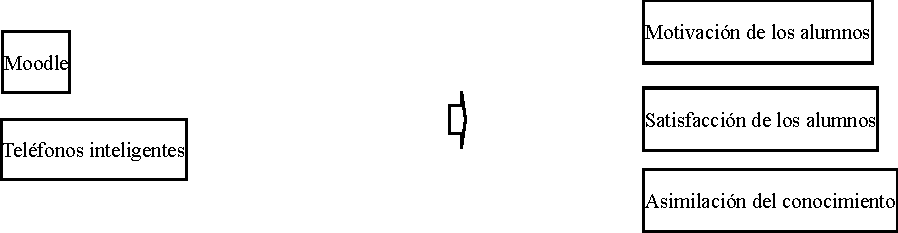
\includegraphics[width=\textwidth]{Image1.pdf}
 \caption{Modelo de estudio.}
 \label{fig01}
 \source{Elaboración propia.}
\end{minipage}
\end{figure}

En la asignatura de Física, los alumnos utilizaron Moodle para la entrega de tareas, la consulta de los contenidos, la revisión de los recursos multimedia y la comunicación. Del mismo modo, los teléfonos inteligentes permitieron el acceso a las plataformas virtuales de aprendizaje, el uso de las aplicaciones móviles y la comunicación desde cualquier lugar.

Actualmente, la Ciencia de Datos permite que los investigadores analicen los fenómenos educativos a través del descubrimiento de nueva información \cite{salas-rueda_use_2021}. De hecho, el empleo de las técnicas regresión lineal, deep learning y árbol de decisión en el campo educativo facilita el análisis, la clasificación y la evaluación de los factores que intervienen en el proceso de enseñanza-aprendizaje.

En este estudio, los algoritmos Machine Learning sobre la regresión lineal y deep learning son utilizados para evaluar las hipótesis. Los sistemas de gestión de aprendizaje facilitan la participación, la interacción y la comunicación entre los alumnos y el educador \cite{karahisar_research_2022, koyuncu_classification_2022}. Por consiguiente, las hipótesis de investigación sobre el uso de Moodle en la asignatura de Física son:

\begin{itemize}
  \item Hipótesis 1: El uso de Moodle influye positivamente la asimilación del conocimiento en el curso Física. 
  \item Hipótesis 2: El uso de Moodle influye positivamente la motivación de los alumnos en el curso Física. 
  \item Hipótesis 3: El uso de Moodle influye positivamente la satisfacción de los estudiantes en el curso Física. 
\end{itemize}

Durante el periodo COVID-19, las universidades y preparatorias utilizaron los dispositivos móviles para establecer la comunicación y ejecutar las actividades a distancia \cite{rysbayeva_students_2022, verawati_enhancing_2022}. Por consiguiente, las hipótesis de investigación sobre el uso de los teléfonos inteligentes en el proceso educativo de la Física son:

\begin{itemize}
  \item Hipótesis 4: El uso de los teléfonos inteligentes influye positivamente la asimilación del conocimiento en el curso Física.
  \item Hipótesis 5: El uso de los teléfonos inteligentes influye positivamente la motivación de los alumnos en el curso Física.
  \item Hipótesis 6: El uso de los teléfonos inteligentes influye positivamente la satisfacción de los estudiantes en el curso Física. 
\end{itemize}

Asimismo, el algoritmo árbol de decisión es utilizado para identificar las condiciones predictivas a través de las características de los alumnos. En esta investigación, los modelos predictivos sobre el empleo de Moodle en el proceso educativo de la Física son:

\begin{itemize}
  \item Modelo Predictivo 1, MP1, sobre el uso de Moodle, las características de los participantes y la asimilación del conocimiento. 
  \item Modelo Predictivo 2, MP2, sobre el uso de Moodle, las características de los participantes y la motivación. 
  \item Modelo Predictivo 3, MP3, sobre el uso de Moodle, las características de los participantes y la satisfacción. 
\end{itemize}

Asimismo, las condiciones predictivas (modelos) sobre el empleo de los teléfonos inteligentes en la asignatura de Física son:

\begin{itemize}
  \item Modelo Predictivo 4, MP4, sobre el uso de los teléfonos inteligentes, las características de los participantes y la asimilación del conocimiento. 
  \item Modelo Predictivo 5, MP5, sobre el uso de los teléfonos inteligentes, las características de los participantes y la motivación. 
  \item Modelo Predictivo 6, MP6, sobre el uso de los teléfonos inteligentes, las características de los participantes y la satisfacción. 
\end{itemize}

\subsection{Recolección de datos}
La recolección de la información se realizó en el mes de diciembre del 2021. La \Cref{tab01} presenta el instrumento de medición, un cuestionario.

%TABELA 1 
\begin{table}[htpb]
\small
\begin{threeparttable}
\caption{Instrumento de medición.}
\label{tab01}
\begin{tabular}{*{3}{l}p{3.5cm}*{3}{l}}
\toprule
No. & Variable & Dimensión & Pregunta & Respuesta & n & \% \\
\midrule
\arrayrulecolor[gray]{.7}
\multirow{6}{*}{1} & \multicolumn{1}{p{1.5cm}}{\multirow{6}{=}{Perfil del estudiante}} & \multirow{2}{*}{Sexo} & \multirow{2}{=}{1. ¿Cuál es tu sexo?} & Hombre & 68 & 64.76 \\
 & & & & Mujer & 37 & 35.24 \\
 \cmidrule{3-7}
 & & \multirow{4}{*}{Edad} & \multirow{4}{*}{2. ¿Cuál es tu edad?} & 16 años & 14 & 13.33 \\
 & & & & 17 años & 83 & 79.05 \\
 & & & & 18 años & 6 & 5.71 \\
 & & & & 19 años & 2 & 1.90 \\
\midrule
\multirow{20}{*}{2} & \multicolumn{1}{p{1.5cm}}{\multirow{20}{*}{Tecnología}} & \multirow{4}{*}{Uso de Moodle} & \multirow{4}{=}{3. El uso de Moodle facilita el proceso de aprendizaje a distancia} & Mucho (1) & 20 & 19.05 \\ 
 & & & & Bastante (2) & 66 & 62.86 \\
 & & & & Poco (3) & 19 & 18.10 \\
 & & & & Muy poco (4) & 0 & 0.00 \\
 \cmidrule{3-7}
 & & \multicolumn{1}{p{3cm}}{\multirow{4}{=}{Uso de teléfonos inteligentes}} & \multirow{4}{=}{4. El uso de los teléfonos inteligentes facilita el proceso de aprendizaje a distancia} & Mucho (1) & 43 & 40.95 \\
 & & & & Bastante (2) & 47 & 44.76 \\
 & & & & Poco (3) & 15 & 14.29 \\
 & & & & Muy poco (4) & 0 & 0.00 \\
 \cmidrule{3-7}
 & & \multicolumn{1}{p{3cm}}{\multirow{4}{=}{Asimilación del conocimiento}} & \multirow{4}{=}{5. Las herramientas tecnológicas facilitan la asimilación del conocimiento en el curso Física} & Mucho (1) & 17 & 16.19 \\
 & & & & Bastante (2) & 43 & 40.95 \\
 & & & & Poco (3) & 38 & 36.19 \\
 & & & & Muy poco (4) & 7 & 6.67 \\
 \cmidrule{3-7}
 & & \multicolumn{1}{p{3cm}}{\multirow{4}{=}{Motivación}} & \multirow{4}{=}{6. Las herramientas tecnológicas incrementan la motivación de los alumnos en el curso Física} & Mucho (1) & 16 & 15.24 \\
 & & & & Bastante (2) & 53 & 50.48 \\
 & & & & Poco (3) & 29 & 27.62 \\
 & & & & Muy poco (4) & 7 & 6.67 \\
 \cmidrule{3-7}
 & & \multicolumn{1}{p{3cm}}{\multirow{4}{=}{Satisfacción}} & \multirow{4}{=}{7. Las herramientas tecnológicas incrementan la satisfacción de los estudiantes en el curso Física} & Mucho (1) & 20 & 19.05 \\
 & & & & Bastante (2) & 42 & 40.00 \\
 & & & & Poco (3) & 33 & 31.43 \\
 & & & & Muy poco (4) & 10 & 9.52 \\
\midrule
\multirow{2}{*}{3} & \multicolumn{1}{p{1.5cm}}{\multirow{2}{=}{Percepción de los estudiantes}} & Moodle & 8. ¿Cuáles son los beneficios de Moodle? & Abierta & - & - \\
 & & Teléfonos inteligentes & 9. ¿Cuáles son los beneficios de los teléfonos inteligentes? & Abierta & - & - \\
\arrayrulecolor{black}
\bottomrule
\end{tabular}
\source{Elaboración propia.}
\end{threeparttable}
\end{table}



La \Cref{tab02} presenta la validación del instrumento de medición.

%TABELA 2

% Please add the following required packages to your document preamble:
% \usepackage{multirow}
\begin{table}
\small
\centering
\caption{Validación del cuestionario}
\label{tab02}
\begin{tabular}{*{6}{l}}
\toprule
    \multicolumn{1}{>{\raggedright\arraybackslash}p{2cm}}{Variable de estudio}         & 
    Dimensión & 
    \multicolumn{1}{>{\raggedright\arraybackslash}p{1.5cm}}{Factor de carga (Load Factor)} & 
    \multicolumn{1}{>{\raggedright\arraybackslash}p{1.5cm}}{Alfa de Cronbach} & 
    \multicolumn{1}{>{\raggedright\arraybackslash}p{1.5cm}}{Average Variance Extracted (AVE)} & 
    \multicolumn{1}{>{\raggedright\arraybackslash}p{1.5cm}}{Composite Reliability (CR)} \\
\toprule
\multirow{5}{*}{Tecnología} & Uso de Moodle                 & 0.524                                                                   & \multirow{5}{*}{0.755} & \multirow{5}{*}{0.530}           & \multirow{5}{*}{0.843}     \\
                            & Uso de teléfonos inteligentes & 0.539                                                                   &                        &                                  &                            \\
                            & Motivación del alumno         & 0.762                                                                   &                        &                                  &                            \\
                            & Asimilación del conocimiento  & 0.875                                                                   &                        &                                  &                            \\
                            & Satisfacción                  & 0.861                                                                   &                        &                                  &                           
\\
\bottomrule
\end{tabular}
\source{Elaboración propia.}
\end{table}


\subsection{Análisis de datos}
RapidMiner permitió el establecimiento de condiciones predictivas (modelos) relacionados con los teléfonos inteligentes, las características de los alumnos y Moodle por medio del algoritmo árbol de decisión (Ver \Cref{fig02}). En este algoritmo Machine Learning, las variables objetivo son la motivación de los alumnos, la asimilación del conocimiento y la satisfacción.

\begin{figure}[htbp]
\centering
\begin{minipage}{.85\textwidth}
 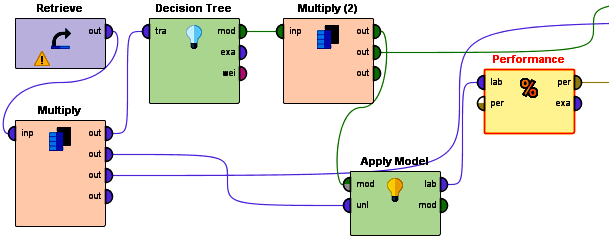
\includegraphics[width=\textwidth]{Image2.png}
 \caption{Algoritmo árbol de decisión en RapidMiner.}
 \label{fig02}
 \source{Elaboración propia.}
\end{minipage}
\end{figure}

Por otro lado, el algoritmo regresión lineal permitió evaluar las hipótesis de este estudio por medio del 70\%, 80\% y 90\% de la muestra. Por otro lado, el 10\%, 20\% y 30\% de la muestra determinó la exactitud de estas regresiones lineales (Ver \Cref{fig03}).

\begin{figure}[htbp]
\centering
\begin{minipage}{.85\textwidth}
 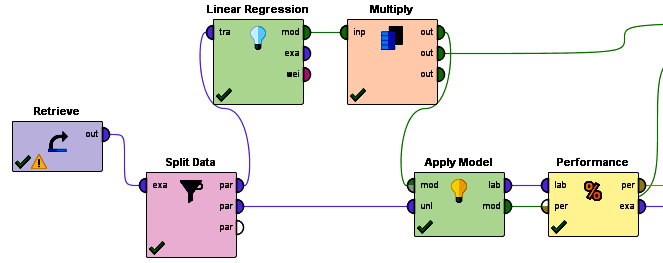
\includegraphics[width=\textwidth]{Image3.png}
 \caption{Algoritmo regresión lineal en RapidMiner.}
 \label{fig03}
 \source{Elaboración propia.}
\end{minipage}
\end{figure}

La \Cref{fig04} muestra los elementos del deep learning utilizados en RapidMiner para analizar cómo influyen el uso de Moodle y los teléfonos inteligentes en la motivación de los alumnos, asimilación del conocimiento y satisfacción en el curso Física. En este algoritmo de Machine Learning se utilizó la activación Tanh, los tamaños de las capas ocultas (50, 50), los ciclos (epochs) = 10, el 70\% de la muestra para la sección de entrenamiento y el 30\% de la muestra para la sección evaluación.

\begin{figure}[htbp]
\centering
\begin{minipage}{.85\textwidth}
 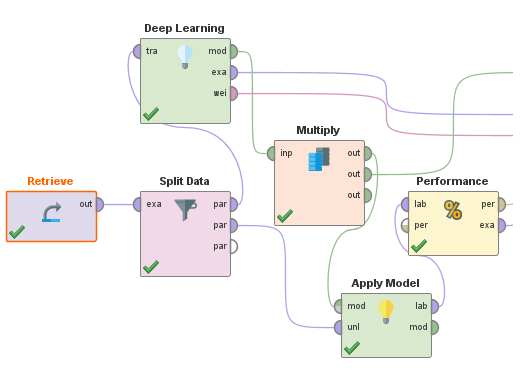
\includegraphics[width=\textwidth]{Image4.png}
 \caption{Algoritmo deep learning en RapidMiner.}
 \label{fig04}
 \source{Elaboración propia.}
\end{minipage}
\end{figure}

Asimismo, la aplicación gratuita llamada Nube-de-Palabras identificó las palabras con mayor frecuencia sobre el uso Moodle y los teléfonos inteligentes en el curso de Física.

\section{Resultados}

Las herramientas tecnológicas facilitan mucho ($n = 17$, 16.19\%), bastante ($n = 43$, 40.95\%), poco ($n = 38$, 36.19\%) y muy poco ($n = 7$, 6.67\%) la asimilación del conocimiento en el curso Física (Ver \Cref{tab01}). Asimismo, las herramientas tecnológicas incrementan mucho ($n = 16$, 15.24\%), bastante ($n = 53$, 50.48\%), poco ($n = 29$, 27.62\%) y muy poco ($n = 7$, 6.67\%) la motivación de los alumnos en el curso Física. Por último, las herramientas tecnológicas incrementan mucho ($n = 20$, 19.05\%), bastante ($n = 42$, 40.00\%), poco ($n = 33$, 31.43\%) y muy poco ($n = 10$, 9.52\%) la satisfacción de los estudiantes en el curso Física.

Los resultados sobre el algoritmo regresión lineal determinan que el uso de Moodle y los teléfonos inteligentes influye positivamente la motivación de los alumnos, la asimilación del conocimiento y la satisfacción de los estudiantes en el curso Física (Ver \Cref{tab03}).

%TABELA 3 
\begin{table}
\setlength{\tabcolsep}{5pt}
\centering
\small
\caption{Resultados del algoritmo Machine Learning sobre la regresión lineal}
\label{tab03}
\begin{tabular}{
    >{\raggedright\arraybackslash}p{3cm}
    >{\raggedright\arraybackslash}p{2.3cm}
    l
    >{\raggedright\arraybackslash}p{1.5cm} 
    ll}
\toprule
Hipótesis de estudio & 
Entrenamiento & 
\multicolumn{1}{>{\raggedright\arraybackslash}p{3cm}}{Algoritmo sobre la regresión lineal} & 
Conclusión & 
\multicolumn{1}{>{\raggedright\arraybackslash}p{1.5cm}}{Error al cuadrado} & 
\multicolumn{1}{>{\raggedright\arraybackslash}p{1.5cm}}{Valor de $p$} \\
\midrule
\arrayrulecolor[gray]{.7}
\multirow{3}{=}{H1: Moodle → asimilación del conocimiento} & 70 \% de muestra & $y = 0.209x + 1.836$ & 0.209. Aceptada. & 0.698 & 0.218 \\
							   & 80 \% de muestra & $y = 0.191x + 1.932$ & 0.191. Aceptada. & 0.514 & 0.211 \\
							   & 90 \% de muestra & $y = 0.227x + 1.867$ & 0.227. Aceptada. & 0.685 & 0.104 \\
\midrule
\multirow{3}{=}{H2: Moodle → motivación} & 70 \% de muestra & $y = 0.386x + 1.545$ & 0.386. Aceptada. & 0.746 & 0.015 \\
					 & 80 \% de muestra & $y = 0.289x + 1.741$ & 0.289. Aceptada. & 0.617 & 0.045 \\
					 & 90 \% de muestra & $y = 0.224x + 1.832$ & 0.224. Aceptada. & 0.678 & 0.094 \\
\midrule
\multirow{3}{=}{H3: Moodle → satisfacción} & 70 \% de muestra & $y = 0.302x + 1.709$ & 0.302. Aceptada. & 0.919 & 0.090 \\
					   & 80 \% de muestra & $y = 0.227x + 1.897$ & 0.227. Aceptada. & 0.861 & 0.153 \\
					   & 90 \% de muestra & $y = 0.198x + 1.915$ & 0.198. Aceptada. & 0.648 & 0.194 \\
\midrule
\multirow{3}{=}{H4: teléfonos inteligentes → asimilación del conocimiento} & 70 \% de muestra & $y = 0.242x + 1.824$ & 0.242. Aceptada. & 0.667 & 0.075 \\
									   & 80 \% de muestra & $y = 0.235x + 1.902$ & 0.235. Aceptada. & 0.458 & 0.084 \\
									   & 90 \% de muestra & $y = 0.214x + 1.945$ & 0.214. Aceptada. & 0.498 & 0.089 \\
\midrule
\multirow{3}{=}{H5: teléfonos inteligentes → motivación} & 70 \% de muestra & $y = 0.326x + 1.732$ & 0.326. Aceptada. & 0.565 & 0.011 \\
							 & 80 \% de muestra & $y = 0.338x + 1.724$ & 0.338. Aceptada. & 0.459 & 0.008 \\
							 & 90 \% de muestra & $y = 0.352x + 1.665$ & 0.352. Aceptada. & 0.528 & 0.003 \\
\midrule
\multirow{3}{=}{H6: teléfonos inteligentes → satisfacción} & 70 \% de muestra & $y = 0.271x + 1.827$ & 0.271. Aceptada. & 0.826 & 0.058 \\
							   & 80 \% de muestra & $y = 0.282x + 1.857$ & 0.282. Aceptada. & 0.786 & 0.046 \\
							   & 90 \% de muestra & $y = 0.278x + 1.824$ & 0.278. Aceptada. & 0.549 & 0.042 \\
\arrayrulecolor{black}
\bottomrule
\end{tabular}
\source{Elaboración propia.}
\end{table}








Del mismo modo, los resultados del algoritmo deep learning indican que el uso de Moodle y los teléfonos inteligentes influye positivamente la motivación de los alumnos, la asimilación del conocimiento y la satisfacción de los estudiantes en el curso Física (Ver \Cref{tab04}).


%TABELA 4 

\begin{table}
\setlength{\tabcolsep}{5pt}
\centering
\small
\caption{Resultados del algoritmo deep learning}
\label{tab04}
\begin{tabular}{*{9}{l}}
\toprule
\multicolumn{1}{>{\raggedright\arraybackslash}p{0.7cm}}{Hipó\-tesis} & 
\multicolumn{1}{>{\raggedright\arraybackslash}p{1cm}}{Entrena\-miento} & 
\multicolumn{1}{>{\raggedright\arraybackslash}p{1cm}}{Capas ocultas} & 
\multicolumn{1}{>{\raggedright\arraybackslash}p{0.8cm}}{Activa\-ción}    & 
\multicolumn{1}{>{\raggedright\arraybackslash}p{1cm}}{Ciclos (epochs)} & 
\multicolumn{1}{>{\raggedright\arraybackslash}p{3cm}}{Algoritmo de Regresión lineal} & Resultado     & 
\multicolumn{1}{>{\raggedright\arraybackslash}p{0.7cm}}{Valor de $p$} & \multicolumn{1}{p{1cm}}{Error al cuadrado} \\
\midrule
H1 & 70 \%  & 50, 50        & Tanh          & 10              & $y = 0.210x + 1.780$    & Aceptada: 0.210 & 0.000   & 0.741             \\
H2 & 70 \%  & 50, 50        & Tanh          & 10              & $y = 0.406x + 1.436$    & Aceptada: 0.406 & 0.000   & 0.732             \\
H3 & 70 \%  & 50, 50        & Tanh          & 10              & $y = 0.238x + 1.843$    & Aceptada: 0.238 & 0.000   & 0.904             \\
H4 & 70 \%  & 50, 50        & Tanh          & 10              & $y = 0.262x + 1.778$    & Aceptada: 0.262 & 0.000   & 0.674             \\
H5 & 70 \%  & 50, 50        & Tanh          & 10              & $y = 0.421x + 1.514$    & Aceptada: 0.421 & 0.000   & 0.532             \\
H6 & 70 \%  & 50, 50        & Tanh & 10              & $y = 0.273x + 1.805$    & Aceptada: 0.273 & 0.000   & 0.828    
\\
\bottomrule
\end{tabular}
\source{Elaboración propia.}
\end{table}



\subsection{Uso de Moodle en el campo educativo}
El uso de Moodle facilita mucho ($n = 20$, 19.05\%), bastante ($n = 66$, 62.86\%) y poco ($n = 19$, 18.10\%) el proceso de aprendizaje a distancia (Ver \Cref{tab01}). Los resultados del algoritmo Machine Learning sobre la regresión lineal con 70\% (0.209, valor de $p = 0.218$), 80\% (0.191, valor de $p = 0.211$) y 90\% (0.227, valor de $p = 0.104$) de la muestra determinan que la Hipótesis 1 es aceptada (Ver \Cref{tab03}). Del mismo modo, el resultado del algoritmo deep learning (0.210, valor $p = 0.000$) con 70\% de la muestra indica que el uso de Moodle influye positivamente la asimilación del conocimiento en el curso Física.

La \Cref{fig05} presenta nueve condiciones sobre el Modelo Predictivo 1. Por ejemplo, si el participante considera que el uso de Moodle facilita mucho el proceso de aprendizaje a distancia y tiene una edad~>~18.5 años entonces las herramientas tecnológicas facilitan mucho la asimilación del conocimiento en el curso Física.

\begin{figure}[htbp]
\centering
\begin{minipage}{.85\textwidth}
 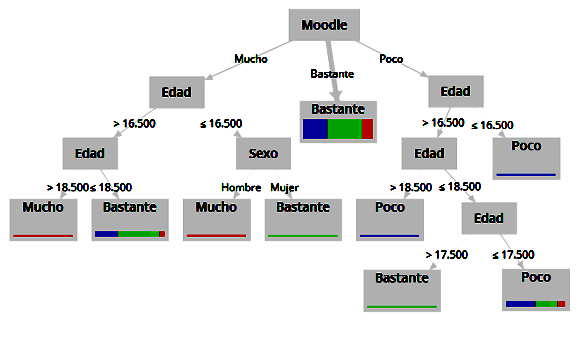
\includegraphics[width=\textwidth]{Image5.png}
 \caption{Condiciones predictivas del Modelo Predictivo 1.}
 \label{fig05}
 \source{Elaboración propia.}
\end{minipage}
\end{figure}

Los resultados del algoritmo Machine Learning sobre la regresión lineal con 70\% (0.386, valor de $p = 0.015$), 80\% (0.289, valor de $p = 0.045$) y 90\% (0.224, valor de $p = 0.094$) de la muestra indican que la Hipótesis 2 es aceptada (Ver \Cref{tab01}). Del mismo modo, el resultado del algoritmo deep learning (0.406, valor de $p = 0.000$) con 70\% de la muestra indica que el uso de Moodle influye positivamente la motivación de los alumnos en el curso Física.

La \Cref{fig06} muestra nueve condiciones sobre el Modelo Predictivo 2. Por ejemplo, si el participante considera que el uso de Moodle facilita mucho el proceso de aprendizaje a distancia y tiene una edad > 17.5 años entonces las herramientas tecnológicas incrementan mucho la motivación en el curso Física.

\begin{figure}[htbp]
\centering
\begin{minipage}{.85\textwidth}
 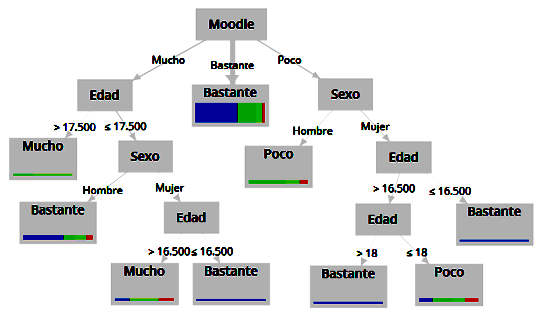
\includegraphics[width=\textwidth]{Image6.png}
 \caption{Condiciones predictivas del Modelo Predictivo 2.}
 \label{fig06}
 \source{Elaboración propia.}
\end{minipage}
\end{figure}

Los resultados del algoritmo Machine Learning sobre la regresión lineal con 70\% (0.302, valor de $p = 0.090$), 80\% (0.227, valor de $p = 0.153$) y 90\% (0.198, valor de $p = 0.194$) de la muestra indican que la Hipótesis 3 es aceptada (Ver \Cref{tab03}). Del mismo modo, el resultado del algoritmo deep learning (0.238, valor de $p = 0.000$) con 70\% de la muestra indica que el uso de Moodle influye positivamente la satisfacción de los alumnos en el curso Física.

La \Cref{fig07} presenta nueve condiciones sobre el Modelo Predictivo 3. Por ejemplo, si el participante considera que el uso de Moodle facilita bastante el proceso de aprendizaje a distancia entonces las herramientas tecnológicas incrementan bastante la satisfacción de los estudiantes en el curso Física.

\begin{figure}[htbp]
\centering
\begin{minipage}{.85\textwidth}
 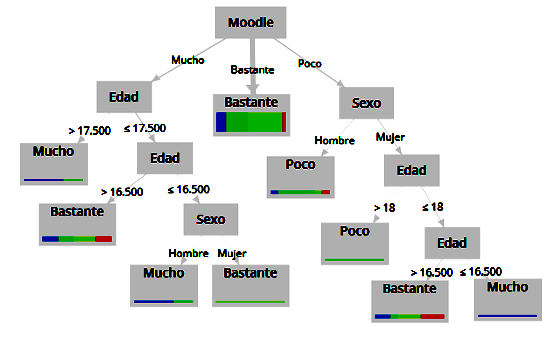
\includegraphics[width=\textwidth]{Image7.png}
 \caption{Condiciones predictivas del Modelo Predictivo 3.}
 \label{fig07}
 \source{Elaboración propia.}
\end{minipage}
\end{figure}

Según los participantes de este estudio, el empleo de Moodle facilitó la consulta y revisión de los contenidos en la asignatura Física y permitió la administración de las tareas desde cualquier lugar.

“Podemos revisar el material previo cuando queramos” (Estudiante 2, 17 años, hombre).

“Que todos podemos recibir el material y las tareas más fácil, además que facilita la visualización de las tareas pendientes y sus entregas” (Estudiante 10, 17 años, hombre).

“Facilidad en la entrega de productos y retroalimentación” (Estudiante 15, 17 años, hombre).

Asimismo, la incorporación de este sistema de gestión de aprendizaje en el curso Física facilitó la retroalimentación de las actividades y permitió la comunicación entre los estudiantes y el educador.

“Se tiene una mejor comunicación alumno-profesor y viceversa, aparte de facilitar la retroalimentación de la clase” (Estudiante 3, 17 años, mujer).

“Facilita la comunicación entre el maestro y el alumno, permite que subamos nuestras tareas de manera más sencilla” (Estudiante 9, 17 años, hombre).

“Tenemos una mayor organización en cuanto a fecha de entrega de trabajos, además de ser un medio para comunicarnos con profesores” (Estudiante 25, 16 años, hombre).

De acuerdo con los alumnos de la UNAM, Moodle promovió la autonomía y permitió el aprendizaje desde cualquier lugar.

“Puedes consultar varias veces algo que no te ha quedado claro” (Estudiante 5, 16 años, hombre).

“Es fácil acceder a ella en cualquier momento en busca de información” (Estudiante 14, 17 años, mujer).

“Poder consultar material expuesto por profesores o inclusive las tareas pasadas con una facilidad impresionante” (Estudiante 33, 17 años, mujer).

En la Escuela Nacional Preparatoria no. 6, este sistema de gestión de aprendizaje permitió que los estudiantes aprendieran a su propio ritmo los temas del curso Física desde cualquier lugar.

“Que nuestros trabajos, las clases y los materiales que se dejan para trabajar se pueden consultar más veces” (Estudiante 12, 17 años, hombre).

 “En los beneficios están: organización de temas vistos y tareas, recordatorios para trabajos y la posibilidad de volver a revisar temas para repasar” (Estudiante 24, 17 años, hombre).
 
“Puedes consultar el material de aprendizaje varias veces, hay una mayor facilidad para organizar tus trabajos y tareas” (Estudiante 35, 17 años, hombre).

La \Cref{fig08} presenta la nube de palabras sobre el empleo de Moodle donde las palabras con mayor frecuencia son tareas ($n = 32$), entrega ($n = 22$), trabajos ($n = 20$), fácil ($n = 18$), organización ($n = 16$), información ($n = 14$), temas ($n = 14$), material ($n = 12$) y consultar ($n = 8$).

\begin{figure}[htbp]
\centering
\begin{minipage}{.85\textwidth}
 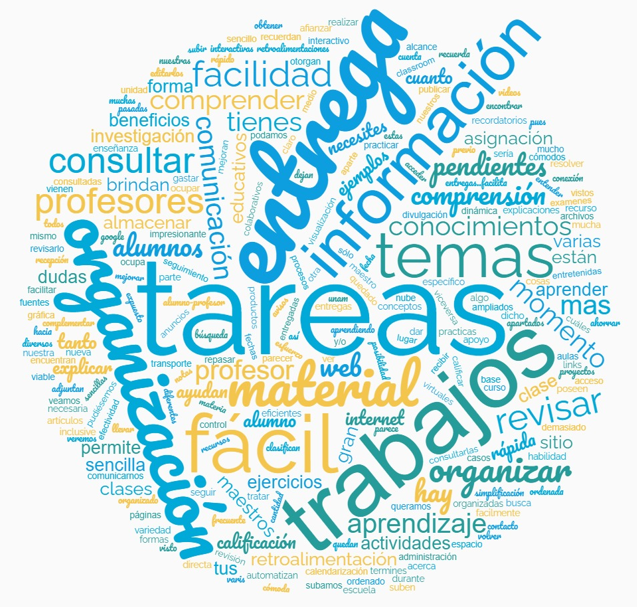
\includegraphics[width=\textwidth]{Image8.png}
 \caption{Nube de palabras sobre el uso de Moodle.}
 \label{fig08}
 \source{Elaboración propia.}
\end{minipage}
\end{figure}

\subsection{Teléfonos inteligentes en el campo educativo}

El uso de los teléfonos inteligentes facilita mucho ($n = 43$, 40.95\%), bastante ($n = 47$, 44.76\%) y poco ($n = 15$, 14.29\%) el proceso de aprendizaje a distancia (Ver \Cref{tab01}). Los resultados del algoritmo Machine Learning sobre la regresión lineal con 70\% (0.242, valor de $p = 0.075$), 80\% (0.235, valor de $p = 0.084$) y 90\% (0.214, valor de $p = 0.089$) de la muestra indican que la Hipótesis 4 es aceptada (Ver \Cref{tab03}). Del mismo modo, el resultado del algoritmo deep learning (0.262, valor de $p = 0.000$) con 70\% de la muestra señala que el uso de los teléfonos inteligentes influye positivamente la asimilación del conocimiento en el curso Física.

Asimismo, la \Cref{fig09} presenta nueve condiciones del Modelo Predictivo 4.  Por ejemplo, si el participante piensa que el uso de los teléfonos inteligentes facilita mucho el proceso de aprendizaje a distancia, tiene una edad ≥ 18.5 años y es hombre entonces las herramientas tecnológicas facilitan mucho la asimilación del conocimiento en el curso Física.

\begin{figure}[htbp]
\centering
\begin{minipage}{.85\textwidth}
 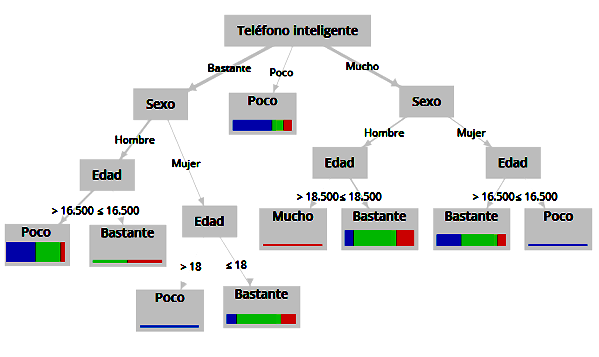
\includegraphics[width=\textwidth]{Image9.png}
 \caption{Condiciones predictivas del Modelo Predictivo 4.}
 \label{fig09}
 \source{Elaboración propia.}
\end{minipage}
\end{figure}

Los resultados del algoritmo Machine Learning sobre la regresión lineal con 70\% (0.326, valor de $p = 0.011$), 80\% (0.338, valor de p = $0.008$) y 90\% (0.352, valor de $p = 0.003$) de la muestra indican que la Hipótesis 5 es aceptada (Ver \Cref{tab03}). Del mismo modo, el resultado del algoritmo deep learning (0.421, valor de $p = 0.000$) con 70\% de la muestra indica que el uso de los teléfonos inteligentes influye positivamente la motivación en el curso Física.

La \Cref{fig10} presenta ocho condiciones del Modelo Predictivo 5. Por ejemplo, si el participante considera que el uso de los teléfonos inteligentes facilita mucho el proceso de aprendizaje a distancia y es mujer entonces las herramientas tecnológicas incrementan bastante la motivación en el curso Física.

\begin{figure}[htbp]
\centering
\begin{minipage}{.85\textwidth}
 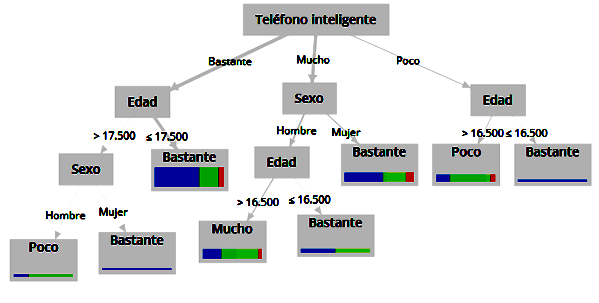
\includegraphics[width=\textwidth]{Imagem10.png}
 \caption{Condiciones predictivas del Modelo Predictivo 5.}
 \label{fig10}
 \source{Elaboración propia.}
\end{minipage}
\end{figure}

Los resultados del algoritmo Machine Learning sobre la regresión lineal con 70\% (0.271, valor de $p = 0.058$), 80\% (0.282, valor de $p = 0.046$) y 90\% (0.278, valor de $p = 0.042$) indican que la Hipótesis 6 es aceptada (Ver \Cref{tab03}). Del mismo modo, el resultado del algoritmo deep learning (0.273, valor de $p = 0.000$) con 70\% de la muestra indica que el uso de los teléfonos inteligentes influye positivamente la satisfacción en el curso Física.

La \Cref{fig11} presenta ocho condiciones del Modelo Predictivo 6. Por ejemplo, si el participante considera que el uso de los teléfonos inteligentes facilita bastante el proceso de aprendizaje a distancia y tiene una edad~$\leq 17.5$ años entonces las herramientas tecnológicas incrementan bastante la satisfacción de los estudiantes en el curso Física.

\begin{figure}[htbp]
\centering
\begin{minipage}{.85\textwidth}
 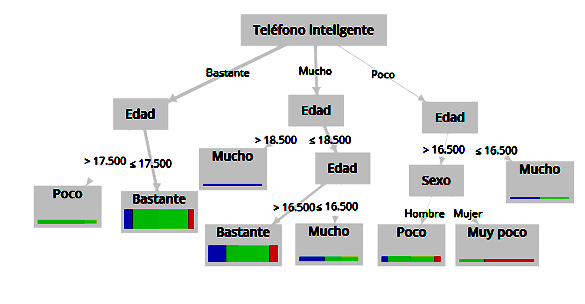
\includegraphics[width=\textwidth]{Image11.png}
 \caption{Condiciones predictivas del Modelo Predictivo 6.}
 \label{fig11}
 \source{Elaboración propia.}
\end{minipage}
\end{figure}

Según los estudiantes del curso Física, el uso de los teléfonos inteligentes en el campo educativo facilitó la comunicación.

“Permiten ponernos en contacto sin importar la distancia” (Estudiante 2, 17 años, hombre).

“La posibilidad de acceder a las clases más fácilmente desde cualquier lugar” (Estudiante 33, 17 años, hombre).

“Es muy fácil poder comunicarse a través de estos dispositivos” (Estudiante 38, 17 años, mujer).

En la Escuela Nacional Preparatoria no. 6, la incorporación de estos dispositivos móviles facilitó el acceso a las herramientas tecnológicas y el aprendizaje a distancia.

“Además de que permiten el aprendizaje a distancia y en cualquier lado, se tiene acceso a las respuestas y a dudas, así como a multitud de programas educativos” (Estudiante 6, 18 años, hombre).

“Facilita el acceso a las aulas virtuales en cualquier lugar y de forma sencilla” (Estudiante 14, 17 años, mujer).
 “Desde el móvil se puede entrar a la plataforma educativa o a una conferencia desde cualquier lado” (Estudiante 20, 17 años, mujer).
 
Los beneficios sobre el empleo de los teléfonos inteligentes en las actividades escolares son la búsqueda de la información, la revisión de los contenidos escolares y la consulta de los recursos multimedia.

“Nos facilitan el acceso a la información” (Estudiante 3, 17 años, mujer).

“El acceso al conocimiento es más rápido y fácil” (Estudiante 8, 18 años hombre).

“Los dispositivos móviles facilitan la búsqueda de la información” (Estudiante 16, 17 años, hombre).

Asimismo, los estudiantes del curso Física utilizaron los teléfonos inteligentes para observar la presentación de los temas de las clases en la modalidad a distancia e intercambiar información en tiempo real durante la pandemia COVID-19.

“Nos permiten conectarnos rápidamente a nuestras clases, permiten tener aplicaciones y permiten visualizar contenido para fortalecer los temas” (Estudiante 9, 17 años, hombre).

 “Con la ayuda de los dispositivos puedo comunicarme con mis compañeros para la elaboración de los trabajos, para conectarme a las clases” (Estudiante 18, 18 años, hombre).
 
“Facilitan la comunicación entre compañeros y profesores” (Estudiante 46, 17 años, mujer).

Asimismo, la \Cref{fig12} presenta la nube de palabras sobre el uso de los teléfonos inteligentes donde las palabras con mayor frecuencia son información (36 veces), clase (18 veces), acceder (14 veces), acceso (12 veces), facilidad (10 veces), herramientas (10 veces), clases (10 veces), dispositivos (10 veces) y aprendizaje (8 veces).

\begin{figure}[htbp]
\centering
\begin{minipage}{.7\textwidth}
 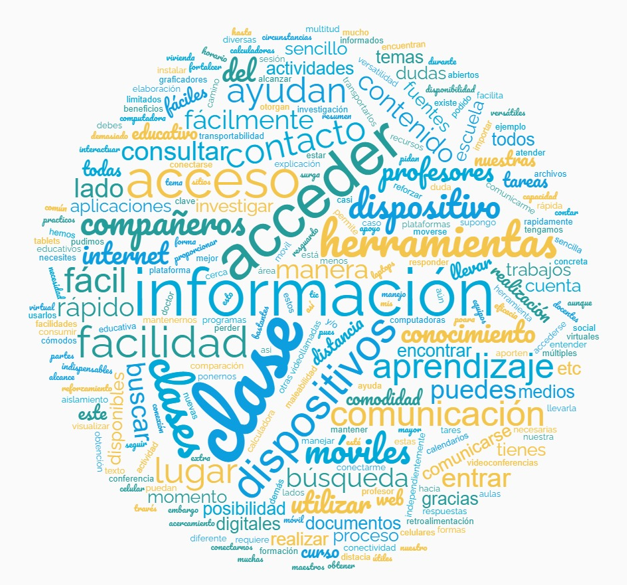
\includegraphics[width=\textwidth]{Image12.png}
 \caption{Nube de palabras sobre el uso de los teléfonos inteligentes.}
 \label{fig12}
 \source{Elaboración propia.}
\end{minipage}
\end{figure}

\section{Discusión}

Durante el periodo del COVID-19, los educadores se apoyaron en los avances tecnológicos para enfrentar los desafíos educativos \cite{area-moreira_blended_2020, cabero-almenara_covid-19:_2020, munoz_arteaga_retos_2022}. Por ejemplo, los beneficios sobre el uso de Moodle en el curso Física son la flexibilidad de tiempo y espacio. En esta investigación, el 57.14\% de los participantes considera que las herramientas tecnológicas facilitan bastante y mucho la asimilación del conocimiento en el curso Física. Por consiguiente, la mayoría de los alumnos tiene una percepción favorable.

Las instituciones educativas emplearon las TIC para actualizar los cursos \cite{cabero-almenara_covid-19:_2020, phamdo_learning_2022}. De hecho, los sistemas de gestión de aprendizaje junto con los dispositivos móviles facilitan la participación de los estudiantes y la realización de las actividades escolares bajo la modalidad a distancia \cite{farsi_investigating_2022}. En la Escuela Nacional Preparatoria no. 6, los teléfonos inteligentes facilitaron y permitieron la comunicación desde cualquier lugar. De hecho, el 65.71\% de los estudiantes piensa que las herramientas tecnológicas incrementan bastante y mucho la motivación en el curso Física. Por consiguiente, la mayoría de los participantes tiene una percepción favorable.

Los avances tecnológicos facilitaron la ejecución de creativas actividades durante el periodo de COVID-19 \cite{area-moreira_blended_2020, farsi_investigating_2022, munoz_arteaga_retos_2022}. Incluso, la incorporación de las herramientas tecnológicas como los sistemas de gestión de aprendizaje y los dispositivos móviles en el campo educativo ayudan a construir nuevos espacios virtuales de enseñanza y aprendizaje \cite{farsi_investigating_2022}. En particular, el empleo de Moodle y los teléfonos inteligentes permitieron actualizar las actividades escolares del curso Física. El 59.05\% de los estudiantes considera que las herramientas tecnológicas incrementan mucho y bastante la satisfacción de los estudiantes en el curso Física. Por consiguiente, la mayoría de los alumnos tienen una percepción favorable.

\subsection{Moodle}

Diversos autores \cite{garcia_integration_2021, phamdo_learning_2022} explican que los sistemas de gestión de aprendizaje permiten el intercambio de ideas. En el curso de Física, Moodle facilitó la revisión de los recursos multimedia y la entrega de las tareas durante el periodo del COVID-19. El 81.90\% de los participantes menciona que el uso de Moodle facilita bastante y mucho el proceso de aprendizaje a distancia. Por lo tanto, la mayoría de los alumnos tiene una percepción favorable.

En la Escuela Nacional Preparatoria no. 6, Moodle facilitó la interacción y comunicación entre los participantes del proceso educativo. Incluso, los resultados del algoritmo regresión lineal sobre la Hipótesis 1 son superiores a 0.189. Del mismo modo, el resultado del algoritmo deep learning señala que la Hipótesis 1 es aceptada.

El algoritmo árbol de decisión determina 9 condiciones sobre el MP1. Este algoritmo del Machine Learning establece las relaciones entre el uso de Moodle y las herramientas tecnológicas para la asimilación del conocimiento por medio del sexo y la edad de los estudiantes.

El educador del curso Física fomentó la autonomía de los alumnos a través de la revisión de los contenidos y el envío de las actividades vía Moodle. Los resultados del algoritmo regresión lineal sobre Hipótesis 2 son superiores a 0.223. Del mismo modo, el resultado del algoritmo deep learning señala que la Hipótesis 2 es aceptada.

El algoritmo árbol de decisión determina 9 condiciones sobre el MP2. Este algoritmo del Machine Learning establece las relaciones entre el uso de Moodle y las herramientas tecnológicas para la motivación por medio del sexo y la edad de los estudiantes.

Según los participantes del curso Física, Moodle promovió el aprendizaje personalizado debido a que este sistema de gestión de aprendizaje facilitó el repaso de los temas en cualquier momento. Los resultados del algoritmo regresión lineal sobre la Hipótesis 3 son superiores a 0.189. Del mismo modo, el resultado del algoritmo deep learning señala que la Hipótesis 3 es aceptada.

El algoritmo árbol de decisión determina 9 condiciones sobre el MP3.  Este algoritmo del Machine Learning establece las relaciones entre el uso de Moodle y las herramientas tecnológicas para la satisfacción por medio del sexo y la edad de los estudiantes.

En la educación a distancia, los sistemas de gestión de aprendizaje facilitan la realización de las actividades escolares desde cualquier lugar \cite{farsi_investigating_2022, galarce-miranda_analysis_2022}.

\subsection{Teléfonos inteligentes}

Los dispositivos móviles facilitaron la realización y entrega de las tareas durante el periodo del COVID-19 \cite{kaminske_cell_2022, perera_university_2021}. En el curso Física, los teléfonos inteligentes permitieron la búsqueda de la información, la revisión de los contenidos escolares y la consulta de los recursos multimedia. El 85.71\% de los estudiantes considera que el uso de estas herramientas tecnológicas facilita bastante y mucho el proceso de aprendizaje a distancia. Por lo tanto, la mayoría de los alumnos tiene una percepción favorable.

Como lo mencionan los estudiantes de la UNAM, el uso de los teléfonos inteligentes facilitó el aprendizaje y la comunicación. De hecho, los resultados del algoritmo regresión lineal sobre la Hipótesis 4 son superiores a 0.209. Del mismo modo, el resultado del algoritmo deep learning señala que la Hipótesis 4 es aceptada.

El algoritmo árbol de decisión determina 9 condiciones predictivas en el MP4. Este algoritmo del Machine Learning establece las relaciones entre el uso de los teléfonos inteligentes y las herramientas tecnológicas para la asimilación del conocimiento por medio del sexo y la edad.

Los estudiantes del curso Física utilizaron los teléfonos inteligentes para acceder a las clases virtuales desde cualquier lugar. Los resultados del algoritmo regresión lineal sobre la Hipótesis 5 son superiores a 0.320. Del mismo modo, el resultado del algoritmo deep learning señala que la Hipótesis 5 es aceptada.

El algoritmo árbol de decisión determina 8 condiciones predictivas en el MP5. Este algoritmo del Machine Learning establece las relaciones entre el uso de los teléfonos inteligentes y las herramientas tecnológicas para la motivación por medio del sexo y la edad de los participantes.

La incorporación de los teléfonos inteligentes facilitó el uso de las herramientas tecnológicas durante el periodo del COVID-19. De hecho, los resultados del algoritmo regresión lineal sobre la Hipótesis 6 son superiores a 0.269. Del mismo modo, el resultado del algoritmo deep learning señala que la Hipótesis 6 es aceptada.

El algoritmo árbol de decisión determina 8 condiciones predictivas en el MP6. Este algoritmo del Machine Learning establece las relaciones entre el uso de los teléfonos inteligentes y las herramientas tecnológicas para la satisfacción por medio del sexo y la edad de los estudiantes.

Por último, los dispositivos móviles facilitan el aprendizaje personalizado y mejora las condiciones de enseñanza en la modalidad a distancia \cite{omirzak_students_2021, verawati_enhancing_2022}.

\section{Conclusión}

Los educadores incorporaron las herramientas tecnológicas en los cursos con el propósito de facilitar el aprendizaje a distancia. En este estudio, los resultados de los algoritmos regresión lineal y deep learning indican que el uso de Moodle y los teléfonos inteligentes influye positivamente la motivación de los alumnos, asimilación del conocimiento y satisfacción de los estudiantes en el curso Física. Asimismo, el algoritmo árbol de decisión determinó seis modelos predictivos considerando el perfil de los participantes.

Esta investigación mixta recomienda la incorporación y el uso de Moodle en el campo educativo porque esta herramienta tecnológica facilitó la entrega de tareas, la consulta de los contenidos, la revisión de los recursos multimedia y la comunicación. Del mismo modo, este trabajo sugiere el empleo de los teléfonos inteligentes en las actividades escolares para el acceso a las plataformas virtuales de aprendizaje, el uso de las aplicaciones móviles y la comunicación desde cualquier lugar.

Las implicaciones de esta investigación mixta son la ejecución de creativas actividades, la realización del proceso educativo a distancia y la organización de espacios virtuales para la enseñanza y el aprendizaje por medio de Moodle y los teléfonos inteligentes. Asimismo, las técnicas de regresión lineal, deep learning y árbol de decisión permiten conocer cuál es el papel que tiene el uso de estas herramientas tecnológicas en el campo educativo. Cabe destacar que el deep learning facilita la creación de modelos matemáticos, funciones lineales, que predicen con gran exactitud el comportamiento de las variables dependientes.

Las limitaciones son las técnicas de Machine Learning utilizadas y el análisis de las herramientas tecnológicas para la asimilación del conocimiento, la motivación y la satisfacción. Los futuros estudios pueden analizar el uso de Moodle y los teléfonos inteligentes para el rol activo y el desarrollo de las habilidades en diversas preparatorias y universidades. Asimismo, los algoritmos Machine Learning sobre los bosques aleatorios y la regresión logística pueden ser empleados para analizar el impacto de estas herramientas tecnológicas considerando el rendimiento académico.

Las líneas de investigación futuras involucran el análisis sobre el uso de las herramientas tecnológicas antes, durante y después de las sesiones presenciales o virtuales. En conclusión, Moodle y los teléfonos inteligentes mejoraron las condiciones de enseñanza-aprendizaje durante el periodo COVID-19 y actualizaron las actividades del curso Física considerando la modalidad de educación a distancia.

\section{Agradecimientos}
Trabajo realizado con el apoyo del Programa UNAM-DGAPA-PAPIME: El Aula del Futuro de la Escuela Nacional Preparatoria 6 (PE106221). Asimismo, se agradece el apoyo proporcionado por el docente del curso Física.


\printbibliography\label{sec-bib}
% if the text is not in Portuguese, it might be necessary to use the code below instead to print the correct ABNT abbreviations [s.n.], [s.l.]
%\begin{portuguese}
%\printbibliography[title={Bibliography}]
%\end{portuguese}


%full list: conceptualization,datacuration,formalanalysis,funding,investigation,methodology,projadm,resources,software,supervision,validation,visualization,writing,review
\begin{contributors}[sec-contributors]
\authorcontribution{Ricardo-Adán Salas-Rueda}[conceptualization,datacuration,formalanalysis,investigation,methodology,validation,writing,review]
\authorcontribution{Jesús Ramírez-Ortega}[funding,investigation,resources,writing,review]
\authorcontribution{Selene-Marisol Martínez-Ramírez}[investigation,writing,review]
\authorcontribution{Clara Alvarado-Zamorano}[investigation,writing,review]
\end{contributors}

\end{document}

